\section{Evaluation and Analysis}

\subsection{Datasets}
We work on a dataset consisting the trajectories of people in Beijing. (We also plan to work on tht following datasetss-)
\begin{itemize}
\item Movebank/Starkey
\item Singapore
\end{itemize}



\subsection{Clustering Effectiveness}

\subsubsection{Silhouette Coefficient}
We show that the proposed algorithm clusters significantly better by using Silhouette Coefficient (SC); a standard metric that shows the effectiveness of clustering. SC is based on the cohesion and the separation of clusters formed. The cohesion ( \textit{a(x)})  is defined as the average distance of x to all other vectors in the same cluster. 
The separation (\textit{b(x)}) is defined as the minimum of the average distances of x to the vectors in other clusters.
Further, the silhouette coefficient of a data point is defined as 
\begin{equation}
s(x)=\frac{b(x)-a(x)}{max(a(x),b(x))}
\end{equation}
The total silhouette coefficient of the dataset is the average over all the points given by
\begin{equation}
SC=\frac{1}{N}\sum_{i=1}^{N}s(x)
\end{equation}
\noindent Ideally, SC is between [-1,1], where values closer to 1 representing better formed clusters. 

\begin{figure}
\centering     
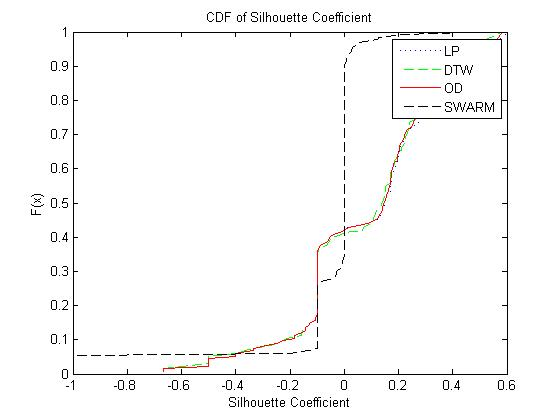
\includegraphics[scale=0.3]{figs/testing_sil.jpg}
\caption{Comparison of silhouette coefficients for different schemes: OD- and LP-based clustering outperform existing mechanism. }
\label{fig:sil_cdf}  
\end{figure}

The CDF plot shows that  DTW is very similar to our approach in terms of clustering effectiveness, but SWARM does a very poor job. 

\subsubsection{Average Trajectories Per Cluster}
Number of clusters with large number of trajectories in it is better (Figure~\ref{fig:avg_cdf} and ~\ref{fig:avgtop_cdf}). 

\begin{figure}[H]
\centering     
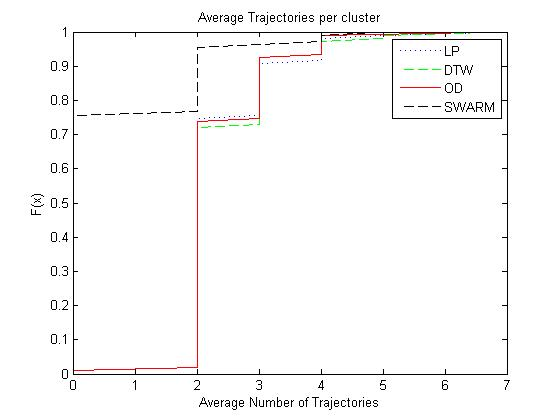
\includegraphics[scale=0.3]{figs/avg.jpg}
\caption{CDF of Average trajectories per cluster for LP-DTW-OD}
\label{fig:avg_cdf}  
\end{figure} 

\begin{figure}[H]
\centering     
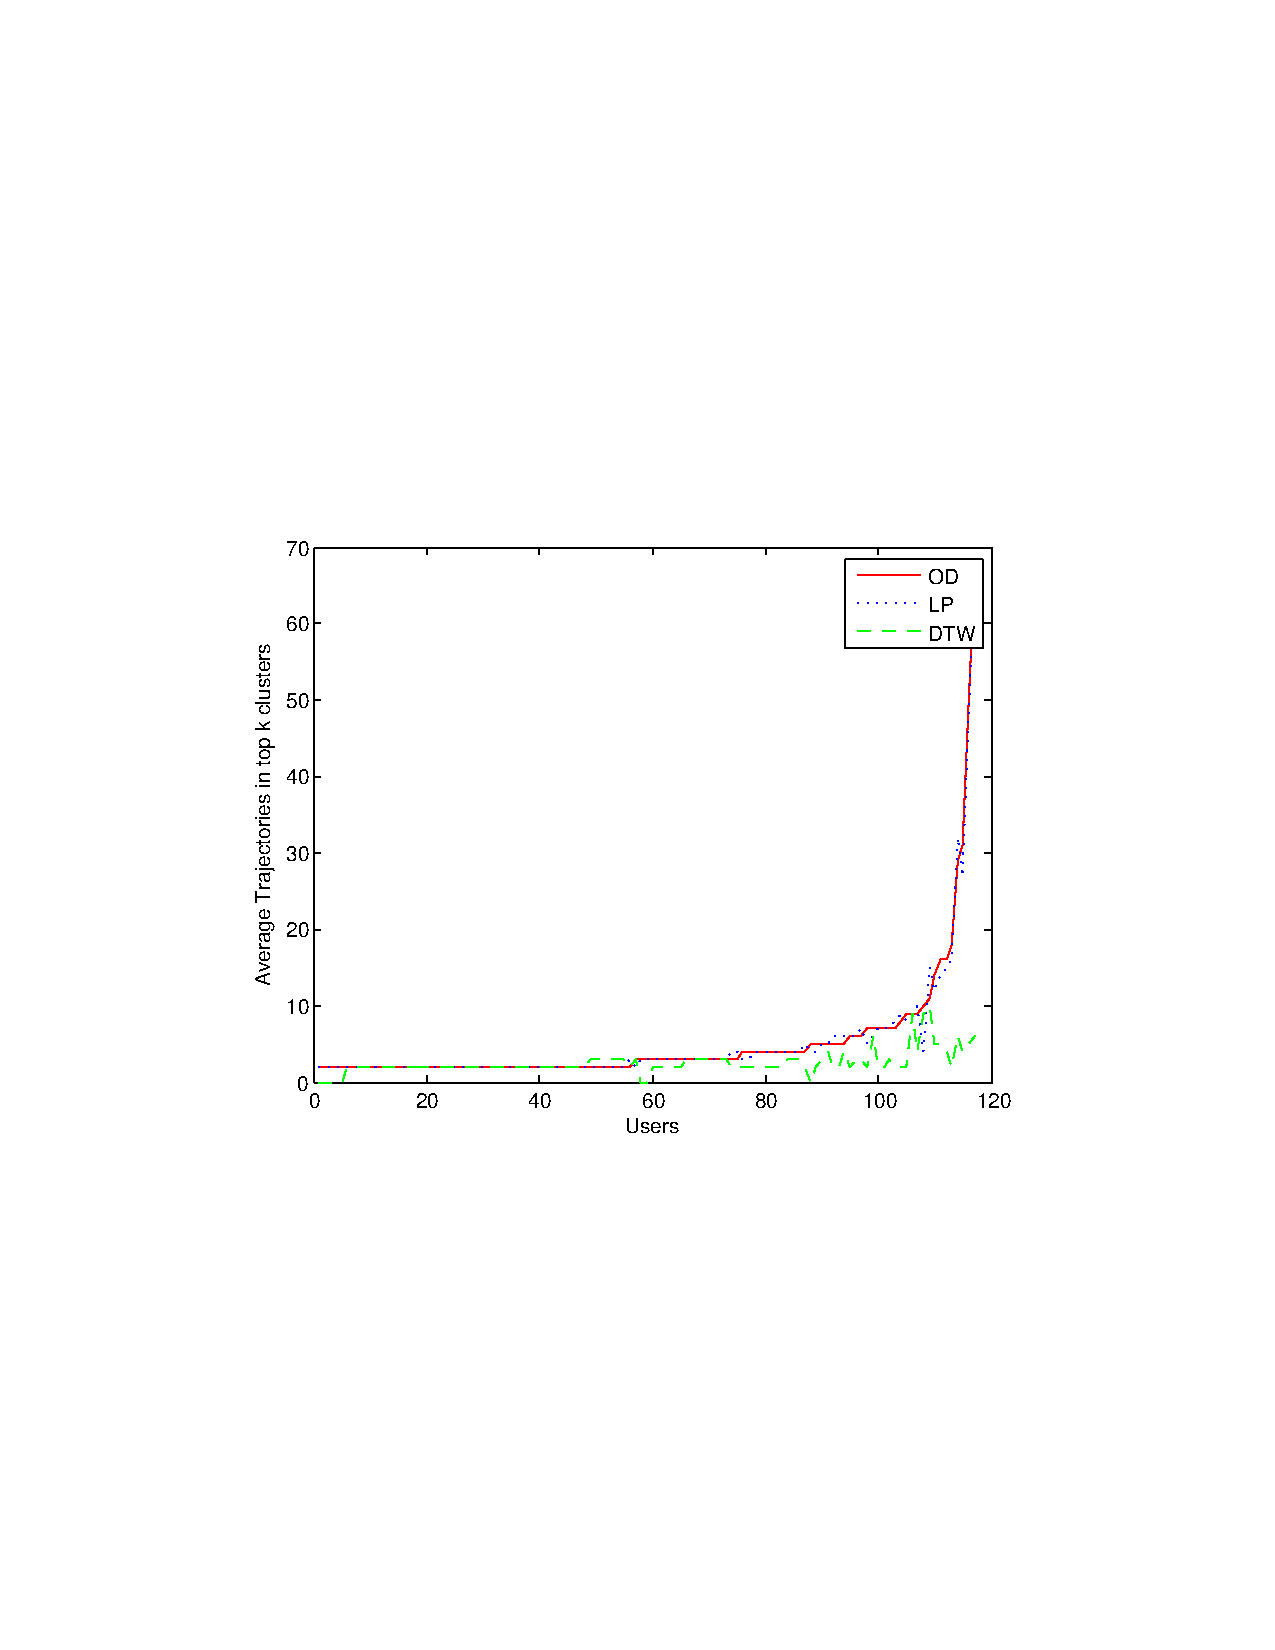
\includegraphics[scale=0.3]{figs/avgtop.jpg}
\caption{CDF of Average trajectories per top-k clusters for LP-DTW-OD}
\label{fig:avgtop_cdf}  
\end{figure} 

\subsection{Computation Time}

\begin{figure}[H]
\centering     
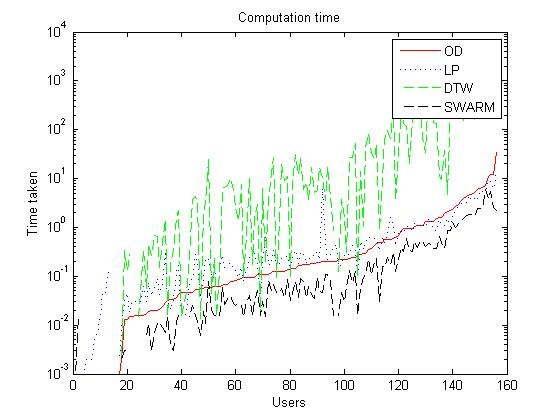
\includegraphics[scale=0.3]{figs/time_log.jpg}
\caption{Computation time  for LP-DTW-OD}
\label{fig:time_cdf}  
\end{figure} 

\subsection{Existing Methods and comparisons} 

We have compared our proposed method with 3 main approaches. The first comparison is made using Dynamic Time Warping as the similarity metric, and clustering based on that matrix. The next is with SWARM, which takes identifies moving clusters. Finally, we compare with TrajClus which is based on partitioning the trajectories into segments, and then clustering over all the partitions. 

Among all the methods, DTW is very close to our method considering the clustering effectiveness, but there are cases where it misses out trajectories that are a part of a meaningful trip summary. On the basis of computation time, our approach is way faster than DTW, because DTW heavily depends on the number of sample points. As the number of sample points increase, the time starts to blow up. 
SWARM is very poor at identifying meaningful summaries, and misses out even very huge clusters for many users. 

\paragraph{Dynamic Time Warping}


Problems with DTW
\begin{itemize}
\item
DTW is not a metric as it violates triangle inequality. This can lead to issues during clustering.Any distance metric d follows triangle inequality if, for any three points, x,y,and z: d(x, z) ≤ d(x, y) + d(y, z).     Figure \ref{fig:dtw_triangleineq} shows an example of the violation of triangle inequality using DTW similarity.
\begin{figure}
\centering     
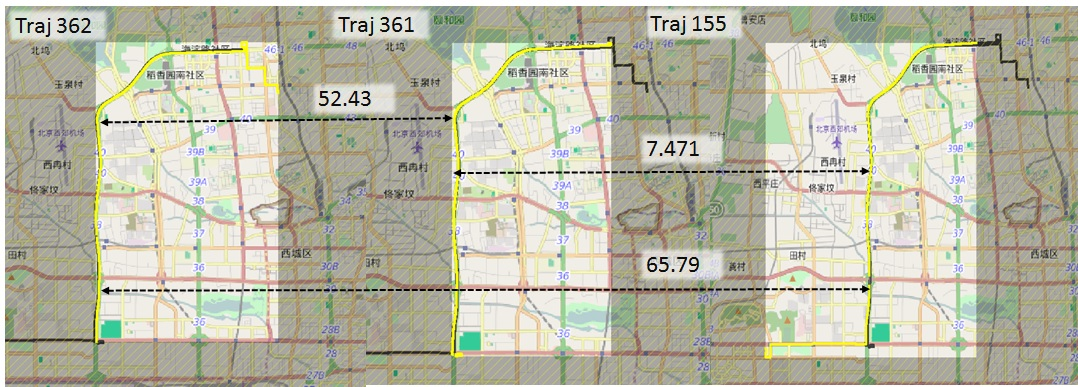
\includegraphics[scale=0.3]{figs/DTW_triangle_ineq.jpg}
\caption{Example of Triangle Inequality Violation using DTW }
\label{fig:dtw_triangleineq}  
\end{figure}

\item 
The biggest concern about DTW is the computation time. When the sample points are very large, it can get to as much as 400 times slower than the proposed approach. If the points are resampled and DTW similarity is computed, it would reduce to the same as pointwise Eucledian distance, and would still be computationally more expensive. Fig \ref{fig:time_dtw_od} shows the computation time differences over all the users for clustering using  DTW and OD similarity measures over all the users

\begin{figure}
\centering     
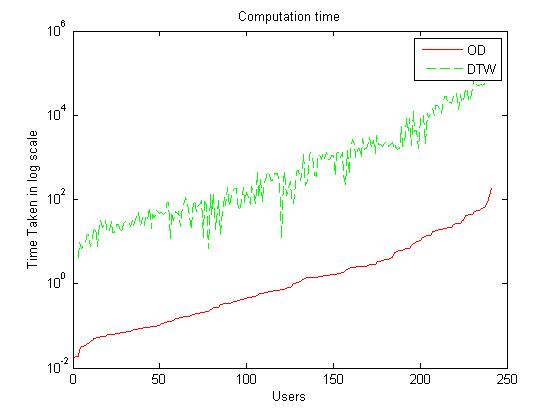
\includegraphics[scale=0.3]{figs/time_dtw_od.jpg}
\caption{Computation time comparison of DTW and OD }
\label{fig:time_dtw_od}  
\end{figure}

\item
As we decrease the number of sample points, the effectiveness of both our proposed method and DTW go down. But the goodness of the clusters returned by DTW decreases more than that of the proposed method. We reduced the number of sample points in each of the trajectories to 90\%,95\%, and 97\% and plotted the silhouette coefficient values using DTW,LP and OD. 

\begin{figure}
\centering     
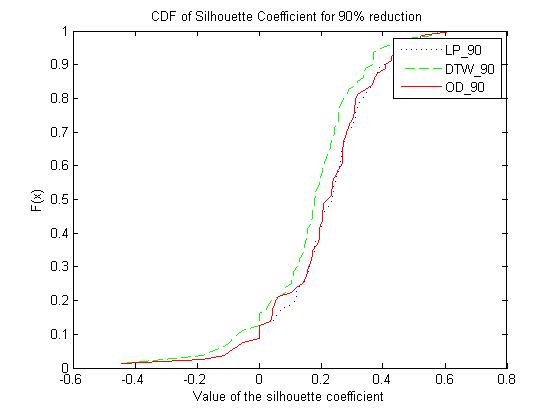
\includegraphics[scale=0.3]{figs/noise_90_cdf.jpg}
\caption{CDF of the silhouette coefficient for 90\% reduction of sample points }
\label{fig:noise_90_cdf}  
\end{figure}

\begin{figure}
\centering     
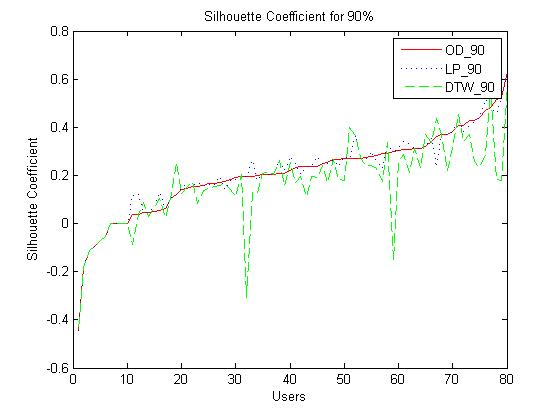
\includegraphics[scale=0.3]{figs/noise_90_sil.jpg}
\caption{Plot of the silhouette coefficient for 90\% reduction of sample points }
\label{fig:noise_90_sil}  
\end{figure}

\begin{figure}
\centering     
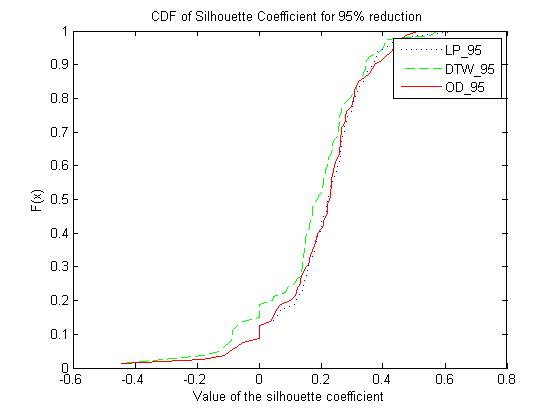
\includegraphics[scale=0.3]{figs/noise_95_cdf.jpg}
\caption{CDF of the silhouette coefficient for 95\% reduction of sample points }
\label{fig:noise_95_cdf}  
\end{figure}

\begin{figure}
\centering     
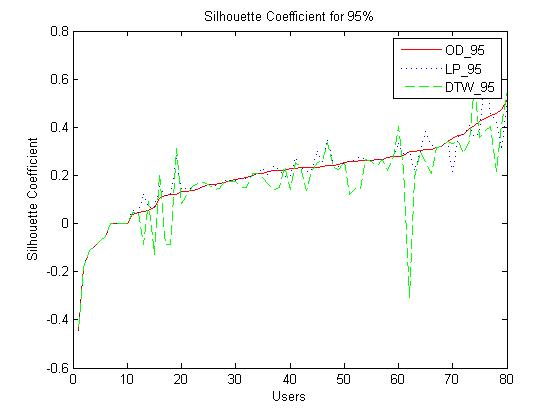
\includegraphics[scale=0.3]{figs/noise_95_sil.jpg}
\caption{Plot of the silhouette coefficient for 95\% reduction of sample points }
\label{fig:noise_95_sil}  
\end{figure}

\begin{figure}
\centering     
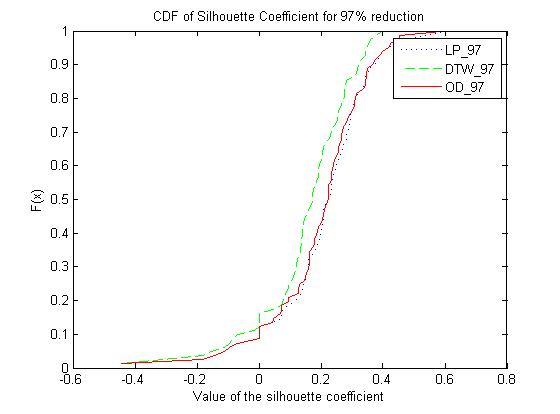
\includegraphics[scale=0.3]{figs/noise_97_cdf.jpg}
\caption{CDF of the silhouette coefficient for 97\% reduction of sample points }
\label{fig:noise_97_cdf}  
\end{figure}

\begin{figure}
\centering     
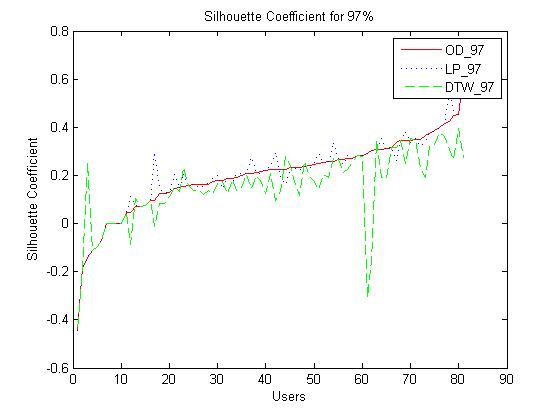
\includegraphics[scale=0.3]{figs/noise_97_sil.jpg}
\caption{Plot of the silhouette coefficient for 97\% reduction of sample points }
\label{fig:noise_97_sil}  
\end{figure}

\end{itemize}

\paragraph{SWARM}

Problems with SWARM 
\begin{itemize}
\item Does not report all the big clusters
\item Dependent a lot on the sample points. If we resample, it would be computationally more expensive than our approach.
\end{itemize}

\paragraph{TrajClus}

TrajClus looks at the sub-trajectory level, and clusters trajectories on the basis of the similarities between those sub-trajectories. In the first phase, it partitions the trajectories into segments, and in the second phase, it clusters the partitions together using a DBSCAN-like technique.The problems with TrajClus are
\begin{itemize}

\item
The similarity measure between any two partitions is defined as a weighted sum of the perpendicular distance, parallel distance and the angular distance between the partitions. Here, three quantities with different units are being merged together, so when two partitions are similar, it is difficult to say which distance contributed to the similarity. Also, this creates a problem in arriving at the neighbourhood parameters. 

\item
 There are two parameters used in this algorithm, \textit{epsilon} and \textit{minLns}. \textit{epsilon} defines the neighourhood reach of each of the partition, and minLns is the minimum number of Partitions required in the neighbourhood for it to be considered as a cluster. The authors suggest a simulated annealing technique to arrive at the value of epsilon , and from that value, further calculate the value of minLns. But, because the algorithm is highly associative, nearly all the partitions end up in one cluster, thus not identifying the correct movement summaries. 
   
\begin{figure}
\centering     
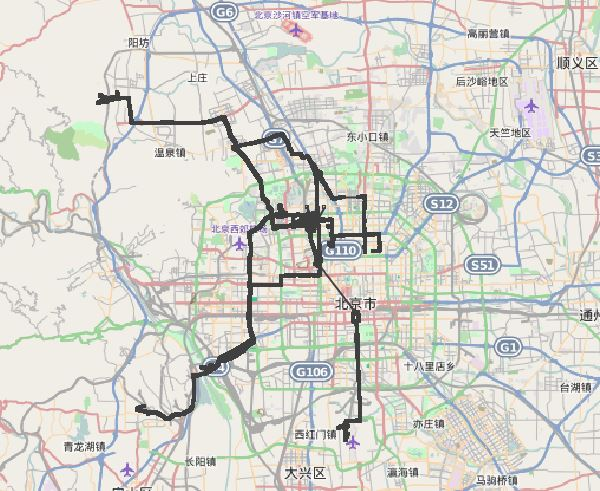
\includegraphics[scale=0.3]{figs/TrajClus_full.jpg}
\caption{All the trajectories of an example user }
\label{fig:TrajClus_full}  
\end{figure}

\begin{figure}
\centering     
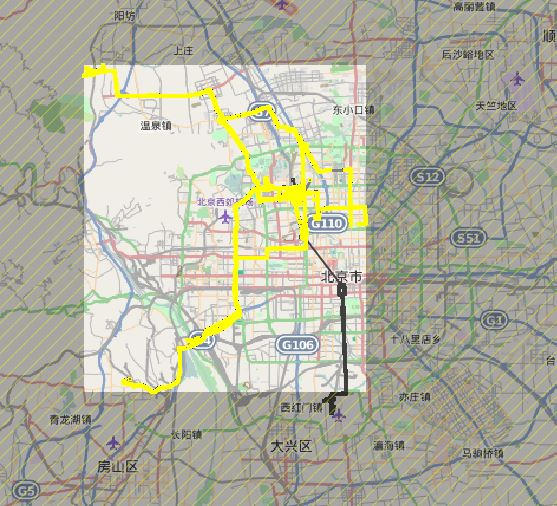
\includegraphics[scale=0.3]{figs/TrajClus_cluster.jpg}
\caption{Cluster reported by TrajClus}
\label{fig:TrajClus_cluster}  
\end{figure}

\item

TrajClus does not give enough weightage to the direction of the line segment. In cases like animal movement or hurricane movement, this makes sense, because there wont be many cases of trajectories in different directions in a flock or cluster. But when it comes to human movement pattern, directions play a very important role in determining the movement summaries of a person. TrajClus overlooks it and clusters two trajectories in different directions in the same cluster.

\begin{figure}
\centering     
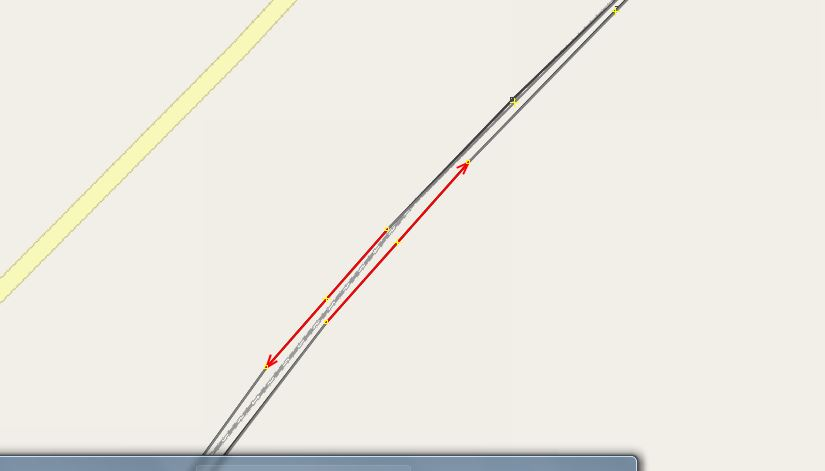
\includegraphics[scale=0.3]{figs/direction.jpg}
\caption{Trajectories with different directions clustered together by TrajClus}
\label{fig:TrajClus_direction}  
\end{figure}

\end{itemize}

\subsection{Next Location Prediction}
Another way to test the summarization of the movement patterns is to test a query trajectory and plot its predicted next location/destination as predicted by all the methods.

The next location prediction is done by the following algorithm:
\paragraph{Explanation of the algo}
For any query trajectory, resample, and compute similarity with the median trajectories of all summary clusters. Report the one with the maximum similarity. 


Let $g(i)$ be the probability of the summary $i$. Given an input traj $t_{\operatorname{in}}$, compute the distance (in meters or so) $d(i,t_{\operatorname{in}})$ between summary $i$ and $t_{\operatorname{in}}$. Now the probability that this sub-trajectory lies within summary $i$ is given by
\begin{eqnarray}
p(i,t_{\operatorname{in}}) = \frac{1}{\sqrt{2 \pi} \sigma_{t}} \mathrm{e}^{-0.5 \left( \frac{d(i,t_{\operatorname{in}})}{\sigma_{t}} \right)}
\end{eqnarray}
Here we assume that the input trajectory is a noisy input from GPS samples. $\sigma_{t}$ is the standard deviation of the sub-trajectory distance. For now take, $\sigma_{t} = \sigma_{p}$, where $\sigma_{p}$ is the standard deviation of the GPS sampling a location (value is 15.61, which is the 95-th percentile of GPS considering 30 m error). It should ideally be standard deviation introduced when we compute distance between 100 points of a path

For each of the methods compared, we plot the CDF of the error of the predicted destination for the Top-3 Closest clusters to each of the query trajectories. Each of the graphs contain 4 plots, each one varying the number of sample points given to the query trajectory. We have plotted the errors for query trajectories with 10\%, 25 \%, 50\% and 90\% of the sample points. 


\begin{figure}
\centering   
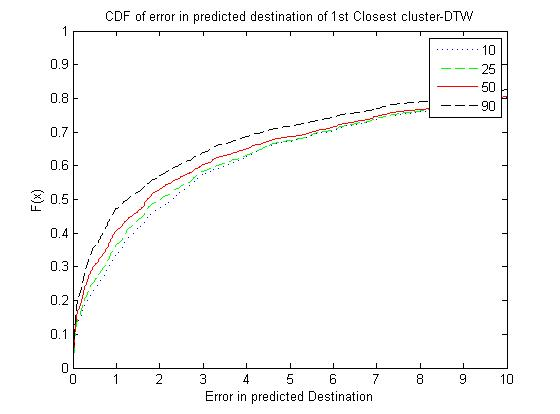
\includegraphics[scale=0.4]{figs/dtw_top.jpg}
\caption{CDF of error in predicted destination for 1st closest cluster using DTW}
\label{fig:dtw_top}  
\end{figure}

\begin{figure}
\centering   
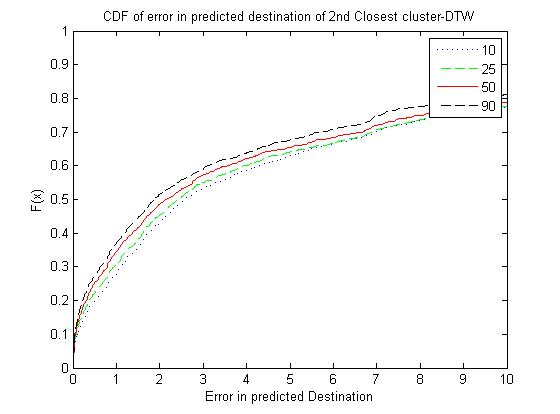
\includegraphics[scale=0.4]{figs/dtw_top2.jpg}
\caption{CDF of error in predicted destination for 2nd closest cluster using DTW}
\label{fig:dtw_top2}  
\end{figure}

\begin{figure}
\centering   
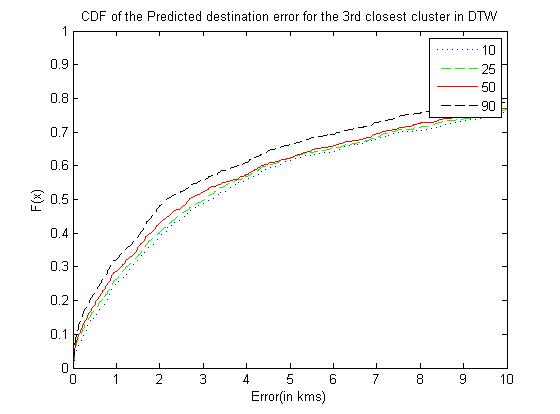
\includegraphics[scale=0.4]{figs/dtw_top3.jpg}
\caption{CDF of error in predicted destination for 3rd closest cluster using DTW}
\label{fig:dtw_top3}  
\end{figure}


\begin{figure}
\centering   
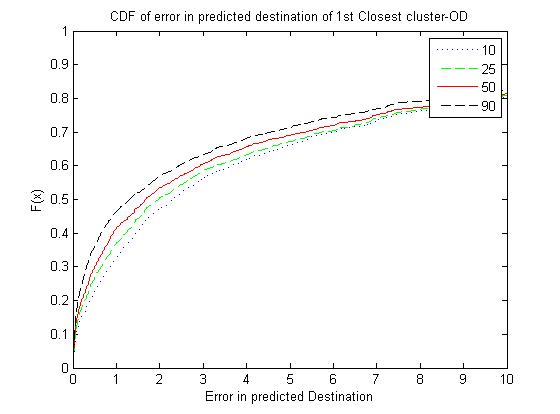
\includegraphics[scale=0.4]{figs/od_top.jpg}
\caption{CDF of error in predicted destination for 1st closest cluster using OD}
\label{fig:od_top}  
\end{figure}

\begin{figure}
\centering   
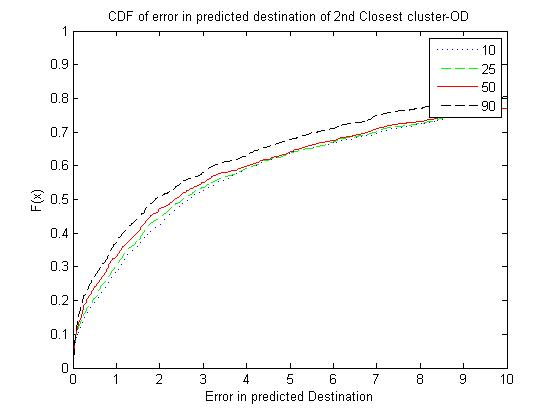
\includegraphics[scale=0.4]{figs/od_top2.jpg}
\caption{CDF of error in predicted destination for 2nd closest cluster using OD}
\label{fig:od_top2}  
\end{figure}

\begin{figure}
\centering   
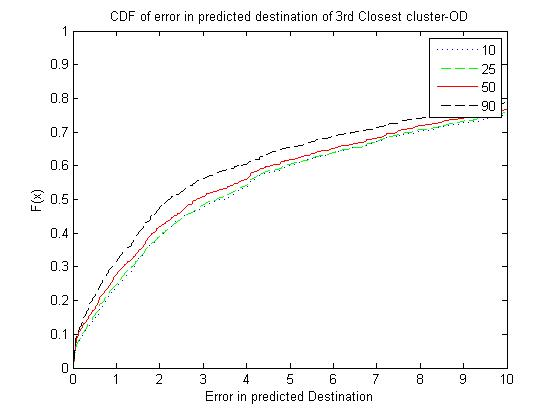
\includegraphics[scale=0.4]{figs/od_top3.jpg}
\caption{CDF of error in predicted destination for 3rd closest cluster using OD}
\label{fig:od_top3}  
\end{figure}


\begin{figure}
\centering   
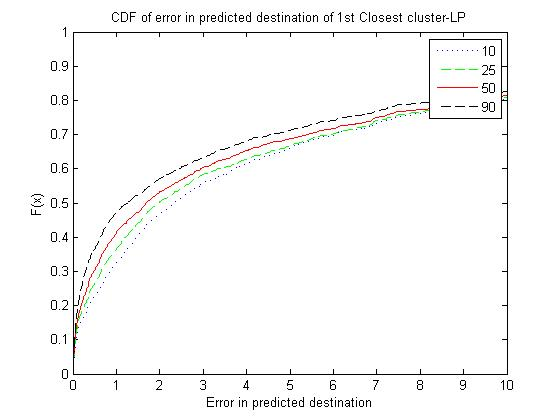
\includegraphics[scale=0.4]{figs/lp_top.jpg}
\caption{CDF of error in predicted destination for 1st closest cluster using LP}
\label{fig:lp_top}  
\end{figure}

\begin{figure}
\centering   
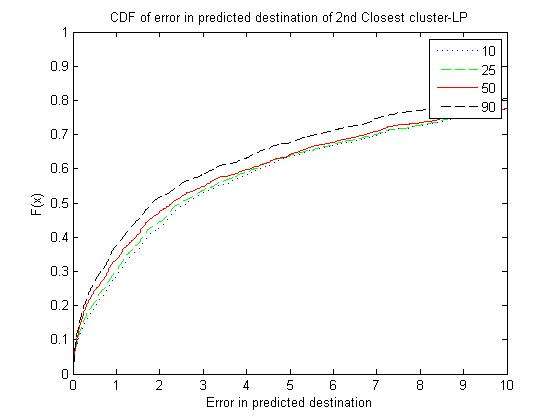
\includegraphics[scale=0.4]{figs/lp_top2.jpg}
\caption{CDF of error in predicted destination for 2nd closest cluster using LP}
\label{fig:lp_top2}  
\end{figure}



\begin{figure}
\centering   
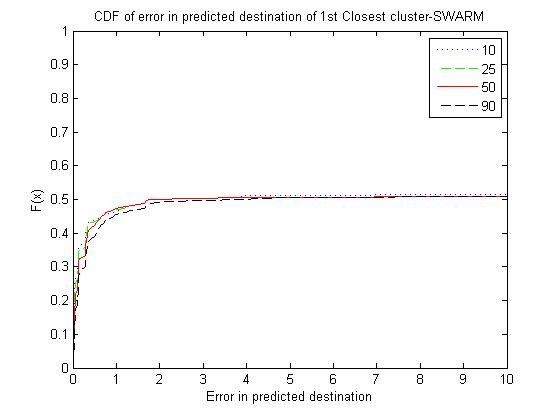
\includegraphics[scale=0.4]{figs/swarm_top.jpg}
\caption{CDF of error in predicted destination for 1st closest cluster using SWARM}
\label{fig:swarm_top}  
\end{figure}

\begin{figure}
\centering   
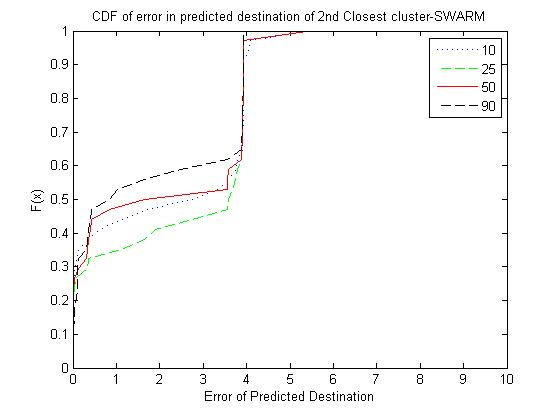
\includegraphics[scale=0.4]{figs/swarm_top2.jpg}
\caption{CDF of error in predicted destination for 2nd closest cluster using SWARM}
\label{fig:swarm_top2}  
\end{figure}

Some of the observations from the next location prediction results are as follows:\\
Our Approach and LP predict the destination of \emph{82\%} of the trajectories with less than 10km error for closest cluster. 
DTW also is very close with prediction \emph{80\%} of the trajectories, but SWARM fares very badly with just \emph{5\%} of the trajectories' destination predicted. SWARM cannot detect the third closest cluster for any of the input trajectories. 




\subsection{Visualization at various granularity }
%\rednote {Remove later if needed}

\begin{figure*}
\centering   
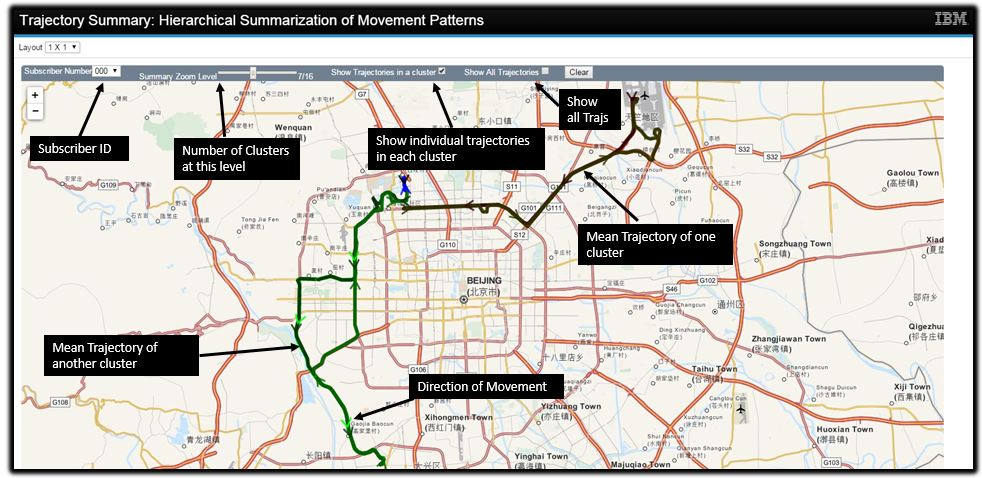
\includegraphics[scale=0.6]{figs/demo.jpg}
\caption{Visualization at various zoom levels}
\label{fig:demo}  
\end{figure*}

\subsection{Case Study: Reported Final Clusters from each method}

We take up a sample case, and show the snapshots of the final clusters as reported by all the different methods. DTW and OD have similar final clusters whereas SWARM reports only final clusters. s


\begin{figure}
\centering     
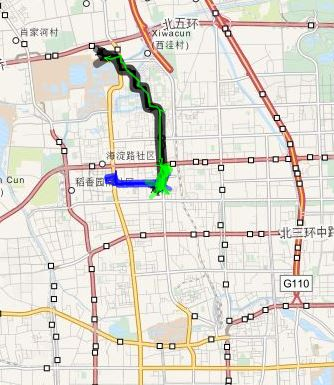
\includegraphics[scale=0.4]{figs/snapshot_swarm.jpg}
\caption{Snapshot of clusters reported by SWARM }
\label{fig:casestudy_swarm}  
\end{figure} 

 
\begin{figure}
\centering     
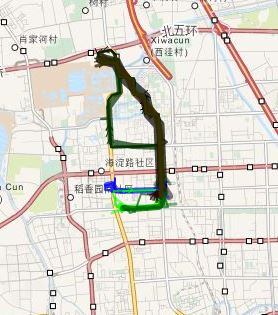
\includegraphics[scale=0.4]{figs/snapshot_od.jpg}
\caption{Snapshot of clusters reported by OD}
\label{fig:casestudy_od}  
\end{figure} 

\begin{figure}
\centering     
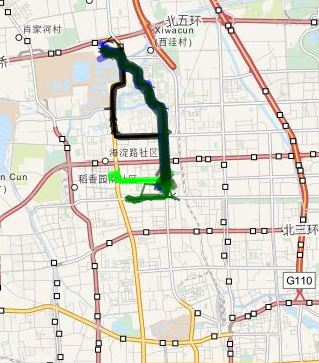
\includegraphics[scale=0.4]{figs/snapshot_dtw.jpg}
\caption{Snapshot of clusters reported by DTW}
\label{fig:casestudy_dtw}  
\end{figure} 

\iffalse
The table below shows the statistics of the top k clusters and the number of trajectories 

\begin{table*}
	\centering
		\begin{tabular}{|c|c|c|c|c|} 
			\hline
			Method&DTW&SWARM&TrajClus&OD\\
			\hline
			Number of Clusters Reported&1&4&0&18\\
			Number of trajectories in top 3 Clusters & 5&36,15,13&0&38,37,29\\
			\hline
		\end{tabular}
	\caption{Comparison for case study}
	\label{tab:case_study}
\end{table*}
\fi